\documentclass[11pt,a4paper]{report}%especifica o tipo de documento que tenciona escrever: carta, artigo, relatório... neste caso é um relatório
% [11pt,a4paper] Define o tamanho principal das letras do documento. caso não especifique uma delas, é assumido 10pt
% a4paper -- Define o tamanho do papel.
\usepackage{float}
\usepackage[portuges]{babel}%Babel -- irá activar automaticamente as regras apropriadas de hifenização para a língua todo o
                                   %-- o texto gerado é automaticamente traduzido para Português.
                                   %  Por exemplo, “chapter” irá passar a “capítulo”, “table of contents” a “conteúdo”.
                                   % portuges -- específica para o Português.
\usepackage[utf8]{inputenc} % define o encoding usado texto fonte (input)--usual "utf8" ou "latin1

\usepackage{graphicx} %permite incluir graficos, tabelas, figuras
\usepackage{url} % para utilizar o comando \url{}
\usepackage{enumerate} %permite escolher, nas listas enumeradas, se os iems sao marcados com letras ou numeros-romanos em vez de numeracao normal

%\usepackage{apalike} % gerar biliografia no estilo 'named' (apalike)

\usepackage{color} % Para escrever em cores
\usepackage{tabularx}

\usepackage{multirow} %tabelas com multilinhas
\usepackage{array} %formatação especial de tabelas em array

\usepackage[pdftex]{hyperref} % transformar as referências internas do seu documento em hiper-ligações.

%Exemplos de fontes -- nao e vulgar mudar o tipo de fonte
%\usepackage{tgbonum} % Fonte de letra: TEX Gyre Bonum
%\usepackage{lmodern} % Fonte de letra: Latin Modern Sans Serif
%\usepackage{helvet}  % Fonte de letra: Helvetica
%\usepackage{charter} % Fonte de letra:Charter

\definecolor{saddlebrown}{rgb}{0.55, 0.27, 0.07} % para definir uma nova cor, neste caso 'saddlebrown'

\usepackage{listings}  % para utilizar blocos de texto verbatim no estilo 'listings'
%paramerização mais vulgar dos blocos LISTING - GENERAL
\lstset{
	basicstyle=\small, %o tamanho das fontes que são usadas para o código
	numbers=left, % onde colocar a numeração da linha
	numberstyle=\tiny, %o tamanho das fontes que são usadas para a numeração da linha
	numbersep=5pt, %distancia entre a numeração da linha e o codigo
	breaklines=true, %define quebra automática de linha
    frame=tB,  % caixa a volta do codigo
	mathescape=true, %habilita o modo matemático
	escapeinside={(*@}{@*)} % se escrever isto  aceita tudo o que esta dentro das marcas e nao altera
}
%
%\lstset{ %
%	language=Java,							% choose the language of the code
%	basicstyle=\ttfamily\footnotesize,		% the size of the fonts that are used for the code
%	keywordstyle=\bfseries,					% set the keyword style
%	%numbers=left,							% where to put the line-numbers
%	numberstyle=\scriptsize,				% the size of the fonts that are used for the line-numbers
%	stepnumber=2,							% the step between two line-numbers. If it's 1 each line
%											% will be numbered
%	numbersep=5pt,							% how far the line-numbers are from the code
%	backgroundcolor=\color{white},			% choose the background color. You must add \usepackage{color}
%	showspaces=false,						% show spaces adding particular underscores
%	showstringspaces=false,					% underline spaces within strings
%	showtabs=false,							% show tabs within strings adding particular underscores
%	frame=none,								% adds a frame around the code
%	%abovecaptionskip=-.8em,
%	%belowcaptionskip=.7em,
%	tabsize=2,								% sets default tabsize to 2 spaces
%	captionpos=b,							% sets the caption-position to bottom
%	breaklines=true,						% sets automatic line breaking
%	breakatwhitespace=false,				% sets if automatic breaks should only happen at whitespace
%	title=\lstname,							% show the filename of files included with \lstinputlisting;
%											% also try caption instead of title
%	escapeinside={\%*}{*)},					% if you want to add a comment within your code
%	morekeywords={*,...}					% if you want to add more keywords to the set
%}

\usepackage{xspace} % deteta se a seguir a palavra tem uma palavra ou um sinal de pontuaçao se tiver uma palavra da espaço, se for um sinal de pontuaçao nao da espaço

\parindent=0pt %espaço a deixar para fazer a  indentação da primeira linha após um parágrafo
\parskip=2pt % espaço entre o parágrafo e o texto anterior

\setlength{\oddsidemargin}{-1cm} %espaço entre o texto e a margem
\setlength{\textwidth}{18cm} %Comprimento do texto na pagina
\setlength{\headsep}{-1cm} %espaço entre o texto e o cabeçalho
\setlength{\textheight}{23cm} %altura do texto na pagina

% comando '\def' usado para definir abreviatura (macros)
% o primeiro argumento é o nome do novo comando e o segundo entre chavetas é o texto original, ou sequência de controle, para que expande
\def\darius{\textsf{Darius}\xspace}
\def\antlr{\texttt{AnTLR}\xspace}
\def\pe{\emph{Publicação Eletrónica}\xspace}
\def\titulo#1{\section{#1}}    %no corpo do documento usa-se na forma '\titulo{MEU TITULO}'
\def\super#1{{\em Supervisor: #1}\\ }
\def\area#1{{\em \'{A}rea: #1}\\[0.2cm]}
\def\resumo{\underline{Resumo}:\\ }

%\input{LPgeneralDefintions} %permite ler de um ficheiro de texto externo mais definições

\title{Engenharia Web\\
        1º/4º ano MEI/MiEI\\
       \textbf{Sidewalk monitoring system }\\ Relatório de IFML
       } %Titulo do documento
%\title{Um Exemplo de Artigo em \LaTeX}
\author{José André Martins Pereira\\ (a82880@alunos.uminho.pt) \and Ricardo André Gomes Petronilho \\ (a81744@alunos.uminho.pt) \and  Rapahel Pinheiro \\ (pg37160@alunos.uminho.pt) 
       } %autores do documento
\date{\today} %data
\usepackage[dvipsnames]{xcolor}

\usepackage{hyperref}
\hypersetup{
    colorlinks=true,
    linkcolor=blue,
    filecolor=magenta,      
    urlcolor=cyan,
}


\begin{document} % corpo do documento

\maketitle % apresentar titulo, autor e data

\section{Introdução}
\hspace{5mm} Na unidade curricular de Engenharia Web, foi proposto o desenvolvimento de um \textit{Sidewalk monitoring system}, onde o principal objetivo consiste em notificar veículos autônomos da presença de pedestres próximos de passadeiras, para que este possam saber se é seguro passar as mesmas.

\hspace{5mm} A primeira fase deste projeto consiste na elaboração de um modelo \textbf{IFML} (utilizando o software Webratio) para a aplicação do SPWS ( Sidewalk Proximity Warning System ), onde se pertende um sistema CRUD (add/see/edit/delete) das passadeiras ("crosswalks"). O registo das passadeiras deve incluir a informação da localização, estado da passagem, número de pedestres/carros na vizinhança. Neste modelo \textbf{IFML}, também se pretende visualizar as distâncias de um pedestre/carro a uma passadeira.

\hspace{5mm} Assim, este relatório serve para complementar/esclarecer algumas decisões tomadas pelo grupo no projeto desenvolvido em Webratio.

\section{Notas e decisões no Webratio}

\subsection{Modelo de domínio}

\begin{figure}[H]
    \centering
    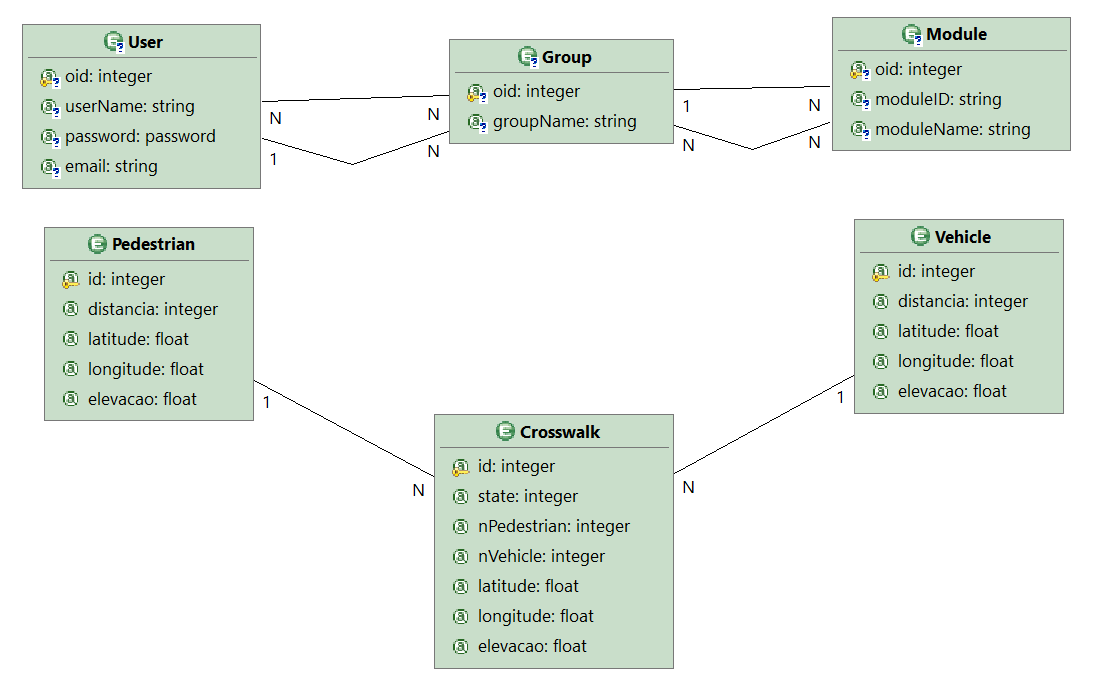
\includegraphics[scale=0.6]{modelo-de-dominio.png}
    \caption{Modelo de domínio.}
    \label{fig:mod_dom}
\end{figure}

\hspace{5mm} Inicialmente foi desenvolvido o modelo de domínio para clarificar as entidades envolventes no sistema e relações entre as mesmas. Note-se que apesar de, neste momento, as entidades: User, Group e Module; não serem usadas, o grupo decidiu permanecer as mesmas no sistema pois serão necessárias para implementar métodos de autenticação entre outros.

\begin{figure}[H]
    \centering
    \includegraphics[scale=0.55]{arquitetura.png}
    \caption{IFML WebRatio.}
    \label{fig:arquitetura}
\end{figure}

\subsection{Create Crosswalk}
\hspace{5mm} A \textit{action create} verifica se existe uma crosswalk com a mesma localização, antes de criar. No entanto, poder-se-á pensar o porquê de verificar a localização e não id. Isso deve-se ao facto de o id ser auto incremental, ou seja, no limite, poderiam existir duas crosswalks na mesma localização, mas com ids diferentes, sendo geograficamente impossível. Assim, para fazer a verificação da localização foi adicionado no \textit{action create} um \textit{selector} com as condições necessárias. 

\hspace{5mm} Tal como foi dito anteriormente o id é auto incremental, ou seja, significa que o formulário para criação de uma nova crosswalk, não necessita de um \textit{text field}, para a inserção do mesmo.

\hspace{5mm} Ainda no create importa realçar que o mesmo não faz update no caso de já existir a passadeira, visto que, preferiu-se separar essas responsabilidades, isto é, existe a action update tal como se irá ver mais adiante. Do mesmo modo, o grupo achou que não era boa ideia fazer o update, visto que o utilizador poderia ter-se enganado, logo achou-se preferível informar do erro.

\begin{figure}[H]
    \centering
    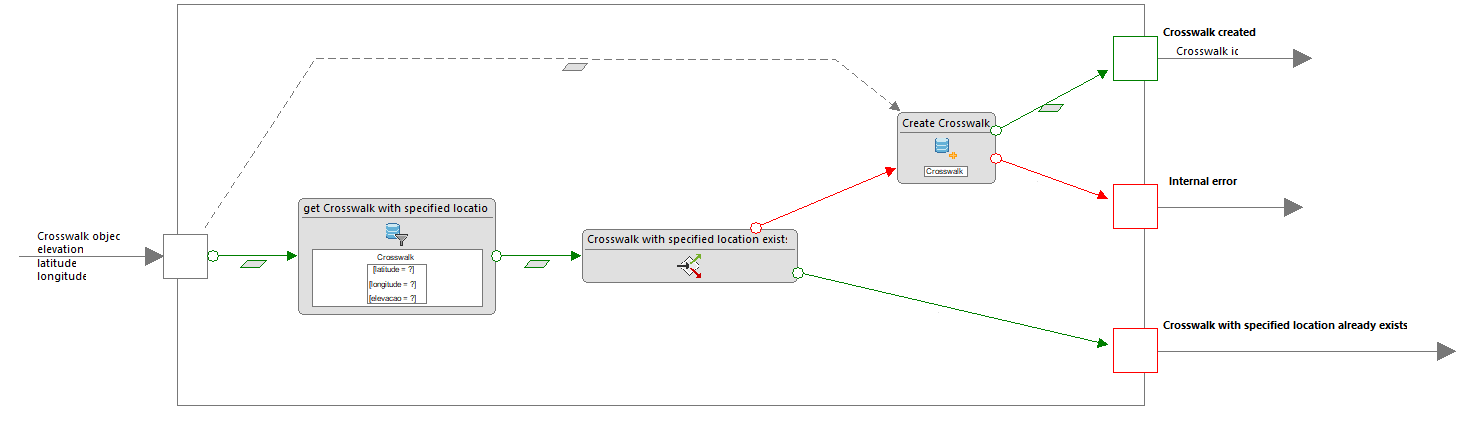
\includegraphics[scale=0.5]{create.PNG}
    \caption{Action create.}
    \label{fig:mod_dom}
\end{figure}

\subsection{Read Crosswalk}
\hspace{5mm} A funcionalidade de Read do \textbf{CRUD}, consiste na aplicação do design pattern \textit{Master and Details}, onde inicialmente se apresenta a lista de passadeiras ("\textit{crosswalks}"). Caso selecione um elemento da lista apresentada, redireciona-se para o \textit{Details} dessa passadeira, onde são listadas todas as informações da mesma, bem como a lista de pedestres/carros na vizinhança, e as suas respetivas distâncias.

\subsection{Update Crosswalk}
\hspace{5mm} Em relação à action update, a mesma começa com o search da passadeira que se pretende atualizar, para verificar se a mesma existe. No entanto, como se está a fazer esta verificação, o grupo aproveitou e fez o preload dos dados da mesma para o formulário do update, utilizando para tal um \textit{selector}, tal como se pode verificar na figura \ref{fig:arquitetura}, na página \textbf{Update Crosswalk}.

\begin{figure}[H]
    \centering
    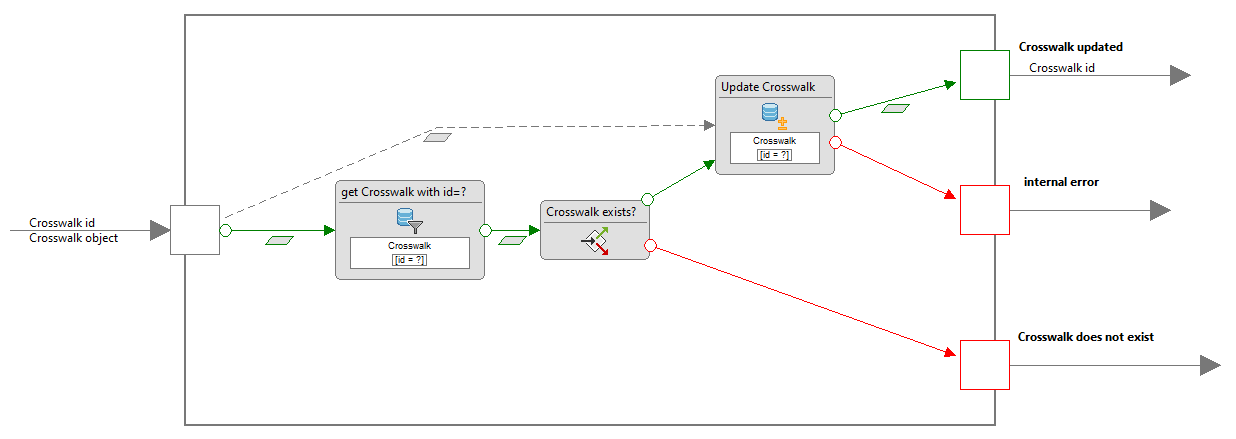
\includegraphics[scale=0.55]{update.PNG}
    \caption{Action update.}
    \label{fig:mod_dom}
\end{figure}


\subsection{Delete Crosswalk}

\hspace{5mm} A action delete é responsável por remover uma Crosswalk do sistema. No momento de remoção verifica-se que a Crosswalk em causa realmente existe, caso contrário notifica-se o utilizador da tentativa de remoção do objeto inexistente. 

\begin{figure}[H]
    \centering
    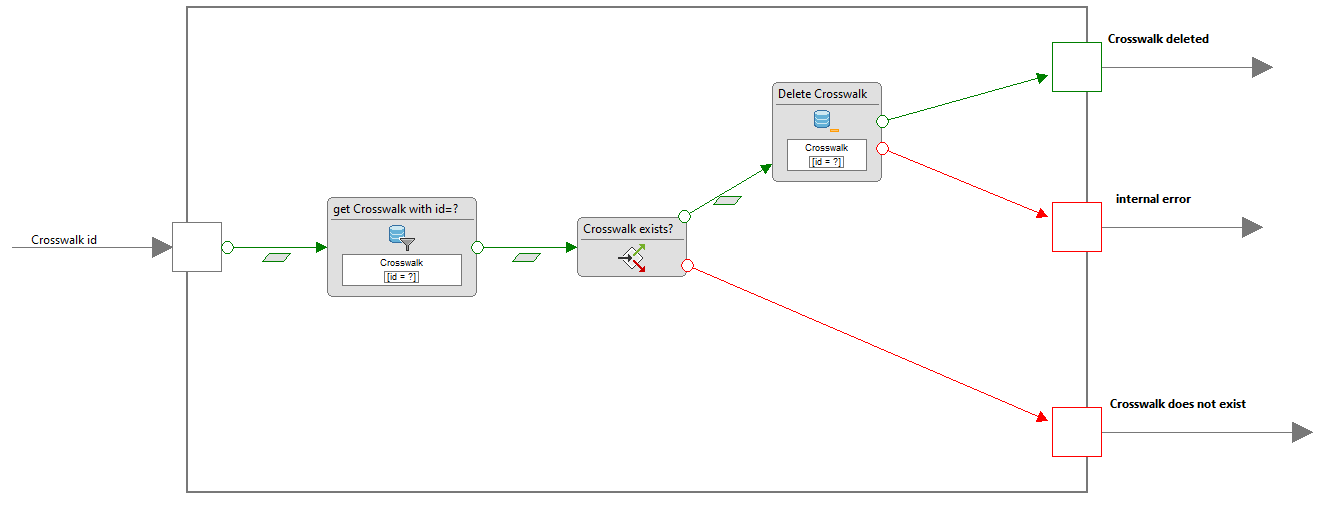
\includegraphics[scale=0.55]{delete.PNG}
    \caption{Action delete.}
    \label{fig:mod_dom}
\end{figure}
    
\subsection{Mensagens de erro}
\hspace{5mm} As actions definidas contém tanto outputs \textbf{OK} como \textbf{KO}. Desta forma, como possíveis mensagens de erro tem-se \textit{"Object does not exist!"}, \textit{"Internal Error!"} e \textit{"Crosswalk with specified location already exists!"}. Assim, criou-se páginas, com as respetivas mensagens, contendo informação abstrata, para que possam ser reutilizadas por diferentes objetos/actions. 

\hspace{5mm} Por outro lado, em caso de sucesso, no create/update, redireciona-se para os details da crosswalk criada/atualizada respetivamente, enquanto que no delete redireciona para a lista de crosswalks, para que o utilizador verifique que foi removida.

\section{Conclusão}
\hspace{5mm} Em suma, conclui-se que os objetivos inicialmente propostos foram cumpridos, isto é, o sistema CRUD para a crosswalk, com as informações localização, estado da passadeira, número de pedestres/carros, bem como a distância dos mesmo à passadeira.

\hspace{5mm} Inicialmente ocorreram dificuldades com a configuração do software WebRatio, tais como a versão necessária do Java (SDK/JRE), bem como a versão compatível do MySQl server.

\hspace{5mm} No entanto, após superar as dificuldades da configuração, a linha de aprendizagem foi produtiva, uma vez que o \textit{Student Guide} fornecido pela equipa docente, explica de forma intuitiva os conceitos, bem como sua aplicação prática.

\hspace{5mm} Assim, conclui-se que a definição do modelo \textbf{IFML} torna-se importante para uma melhor percepção da estrutura da aplicação, bem como do fluxo comportamental da mesma.

\end{document}

